% Created by tikzDevice version 0.12
% !TEX encoding = UTF-8 Unicode
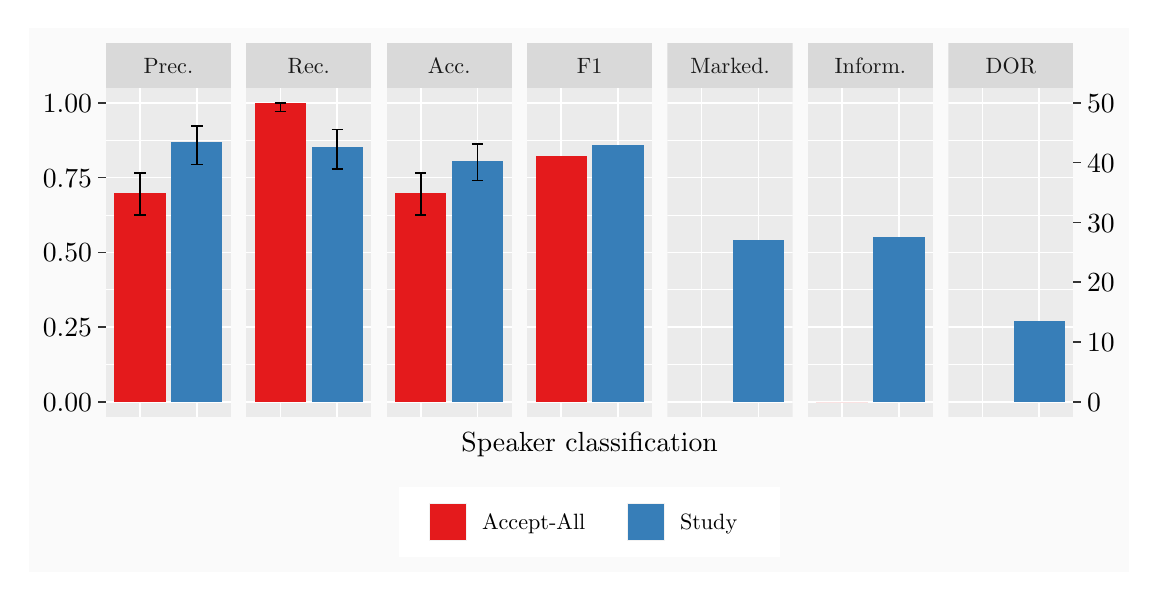
\begin{tikzpicture}[x=1pt,y=1pt]
\definecolor{fillColor}{RGB}{255,255,255}
\path[use as bounding box,fill=fillColor,fill opacity=0.00] (0,0) rectangle (398.34,196.94);
\begin{scope}
\path[clip] (  0.00,  0.00) rectangle (398.34,196.94);
\definecolor{drawColor}{RGB}{255,255,255}
\definecolor{fillColor}{gray}{0.98}

\path[draw=drawColor,line width= 0.6pt,line join=round,line cap=round,fill=fillColor] (  0.00,  0.00) rectangle (398.34,196.94);
\end{scope}
\begin{scope}
\path[clip] ( 28.22, 56.29) rectangle ( 73.46,175.18);
\definecolor{fillColor}{gray}{0.92}

\path[fill=fillColor] ( 28.22, 56.29) rectangle ( 73.46,175.18);
\definecolor{drawColor}{RGB}{255,255,255}

\path[draw=drawColor,line width= 0.3pt,line join=round] ( 28.22, 75.20) --
	( 73.46, 75.20);

\path[draw=drawColor,line width= 0.3pt,line join=round] ( 28.22,102.22) --
	( 73.46,102.22);

\path[draw=drawColor,line width= 0.3pt,line join=round] ( 28.22,129.25) --
	( 73.46,129.25);

\path[draw=drawColor,line width= 0.3pt,line join=round] ( 28.22,156.27) --
	( 73.46,156.27);

\path[draw=drawColor,line width= 0.6pt,line join=round] ( 28.22, 61.69) --
	( 73.46, 61.69);

\path[draw=drawColor,line width= 0.6pt,line join=round] ( 28.22, 88.71) --
	( 73.46, 88.71);

\path[draw=drawColor,line width= 0.6pt,line join=round] ( 28.22,115.74) --
	( 73.46,115.74);

\path[draw=drawColor,line width= 0.6pt,line join=round] ( 28.22,142.76) --
	( 73.46,142.76);

\path[draw=drawColor,line width= 0.6pt,line join=round] ( 28.22,169.78) --
	( 73.46,169.78);

\path[draw=drawColor,line width= 0.6pt,line join=round] ( 40.56, 56.29) --
	( 40.56,175.18);

\path[draw=drawColor,line width= 0.6pt,line join=round] ( 61.12, 56.29) --
	( 61.12,175.18);
\definecolor{fillColor}{RGB}{228,26,28}

\path[fill=fillColor] ( 31.31, 61.69) rectangle ( 49.81,137.23);
\definecolor{fillColor}{RGB}{55,126,184}

\path[fill=fillColor] ( 51.87, 61.69) rectangle ( 70.38,155.49);
\definecolor{drawColor}{RGB}{0,0,0}

\path[draw=drawColor,line width= 0.6pt,line join=round] ( 59.07,161.40) --
	( 63.18,161.40);

\path[draw=drawColor,line width= 0.6pt,line join=round] ( 61.12,161.40) --
	( 61.12,147.53);

\path[draw=drawColor,line width= 0.6pt,line join=round] ( 59.07,147.53) --
	( 63.18,147.53);

\path[draw=drawColor,line width= 0.6pt,line join=round] ( 38.50,144.44) --
	( 42.62,144.44);

\path[draw=drawColor,line width= 0.6pt,line join=round] ( 40.56,144.44) --
	( 40.56,129.28);

\path[draw=drawColor,line width= 0.6pt,line join=round] ( 38.50,129.28) --
	( 42.62,129.28);
\end{scope}
\begin{scope}
\path[clip] ( 78.96, 56.29) rectangle (124.20,175.18);
\definecolor{fillColor}{gray}{0.92}

\path[fill=fillColor] ( 78.96, 56.29) rectangle (124.20,175.18);
\definecolor{drawColor}{RGB}{255,255,255}

\path[draw=drawColor,line width= 0.3pt,line join=round] ( 78.96, 75.20) --
	(124.20, 75.20);

\path[draw=drawColor,line width= 0.3pt,line join=round] ( 78.96,102.22) --
	(124.20,102.22);

\path[draw=drawColor,line width= 0.3pt,line join=round] ( 78.96,129.25) --
	(124.20,129.25);

\path[draw=drawColor,line width= 0.3pt,line join=round] ( 78.96,156.27) --
	(124.20,156.27);

\path[draw=drawColor,line width= 0.6pt,line join=round] ( 78.96, 61.69) --
	(124.20, 61.69);

\path[draw=drawColor,line width= 0.6pt,line join=round] ( 78.96, 88.71) --
	(124.20, 88.71);

\path[draw=drawColor,line width= 0.6pt,line join=round] ( 78.96,115.74) --
	(124.20,115.74);

\path[draw=drawColor,line width= 0.6pt,line join=round] ( 78.96,142.76) --
	(124.20,142.76);

\path[draw=drawColor,line width= 0.6pt,line join=round] ( 78.96,169.78) --
	(124.20,169.78);

\path[draw=drawColor,line width= 0.6pt,line join=round] ( 91.30, 56.29) --
	( 91.30,175.18);

\path[draw=drawColor,line width= 0.6pt,line join=round] (111.86, 56.29) --
	(111.86,175.18);
\definecolor{fillColor}{RGB}{228,26,28}

\path[fill=fillColor] ( 82.05, 61.69) rectangle (100.55,169.78);
\definecolor{fillColor}{RGB}{55,126,184}

\path[fill=fillColor] (102.61, 61.69) rectangle (121.12,153.96);
\definecolor{drawColor}{RGB}{0,0,0}

\path[draw=drawColor,line width= 0.6pt,line join=round] (109.81,160.15) --
	(113.92,160.15);

\path[draw=drawColor,line width= 0.6pt,line join=round] (111.86,160.15) --
	(111.86,145.85);

\path[draw=drawColor,line width= 0.6pt,line join=round] (109.81,145.85) --
	(113.92,145.85);

\path[draw=drawColor,line width= 0.6pt,line join=round] ( 89.24,169.78) --
	( 93.36,169.78);

\path[draw=drawColor,line width= 0.6pt,line join=round] ( 91.30,169.78) --
	( 91.30,166.59);

\path[draw=drawColor,line width= 0.6pt,line join=round] ( 89.24,166.59) --
	( 93.36,166.59);
\end{scope}
\begin{scope}
\path[clip] (129.70, 56.29) rectangle (174.94,175.18);
\definecolor{fillColor}{gray}{0.92}

\path[fill=fillColor] (129.70, 56.29) rectangle (174.94,175.18);
\definecolor{drawColor}{RGB}{255,255,255}

\path[draw=drawColor,line width= 0.3pt,line join=round] (129.70, 75.20) --
	(174.94, 75.20);

\path[draw=drawColor,line width= 0.3pt,line join=round] (129.70,102.22) --
	(174.94,102.22);

\path[draw=drawColor,line width= 0.3pt,line join=round] (129.70,129.25) --
	(174.94,129.25);

\path[draw=drawColor,line width= 0.3pt,line join=round] (129.70,156.27) --
	(174.94,156.27);

\path[draw=drawColor,line width= 0.6pt,line join=round] (129.70, 61.69) --
	(174.94, 61.69);

\path[draw=drawColor,line width= 0.6pt,line join=round] (129.70, 88.71) --
	(174.94, 88.71);

\path[draw=drawColor,line width= 0.6pt,line join=round] (129.70,115.74) --
	(174.94,115.74);

\path[draw=drawColor,line width= 0.6pt,line join=round] (129.70,142.76) --
	(174.94,142.76);

\path[draw=drawColor,line width= 0.6pt,line join=round] (129.70,169.78) --
	(174.94,169.78);

\path[draw=drawColor,line width= 0.6pt,line join=round] (142.04, 56.29) --
	(142.04,175.18);

\path[draw=drawColor,line width= 0.6pt,line join=round] (162.60, 56.29) --
	(162.60,175.18);
\definecolor{fillColor}{RGB}{228,26,28}

\path[fill=fillColor] (132.78, 61.69) rectangle (151.29,137.23);
\definecolor{fillColor}{RGB}{55,126,184}

\path[fill=fillColor] (153.35, 61.69) rectangle (171.85,148.90);
\definecolor{drawColor}{RGB}{0,0,0}

\path[draw=drawColor,line width= 0.6pt,line join=round] (160.54,154.90) --
	(164.66,154.90);

\path[draw=drawColor,line width= 0.6pt,line join=round] (162.60,154.90) --
	(162.60,141.75);

\path[draw=drawColor,line width= 0.6pt,line join=round] (160.54,141.75) --
	(164.66,141.75);

\path[draw=drawColor,line width= 0.6pt,line join=round] (139.98,144.44) --
	(144.09,144.44);

\path[draw=drawColor,line width= 0.6pt,line join=round] (142.04,144.44) --
	(142.04,129.28);

\path[draw=drawColor,line width= 0.6pt,line join=round] (139.98,129.28) --
	(144.09,129.28);
\end{scope}
\begin{scope}
\path[clip] (180.44, 56.29) rectangle (225.68,175.18);
\definecolor{fillColor}{gray}{0.92}

\path[fill=fillColor] (180.44, 56.29) rectangle (225.68,175.18);
\definecolor{drawColor}{RGB}{255,255,255}

\path[draw=drawColor,line width= 0.3pt,line join=round] (180.44, 75.20) --
	(225.68, 75.20);

\path[draw=drawColor,line width= 0.3pt,line join=round] (180.44,102.22) --
	(225.68,102.22);

\path[draw=drawColor,line width= 0.3pt,line join=round] (180.44,129.25) --
	(225.68,129.25);

\path[draw=drawColor,line width= 0.3pt,line join=round] (180.44,156.27) --
	(225.68,156.27);

\path[draw=drawColor,line width= 0.6pt,line join=round] (180.44, 61.69) --
	(225.68, 61.69);

\path[draw=drawColor,line width= 0.6pt,line join=round] (180.44, 88.71) --
	(225.68, 88.71);

\path[draw=drawColor,line width= 0.6pt,line join=round] (180.44,115.74) --
	(225.68,115.74);

\path[draw=drawColor,line width= 0.6pt,line join=round] (180.44,142.76) --
	(225.68,142.76);

\path[draw=drawColor,line width= 0.6pt,line join=round] (180.44,169.78) --
	(225.68,169.78);

\path[draw=drawColor,line width= 0.6pt,line join=round] (192.78, 56.29) --
	(192.78,175.18);

\path[draw=drawColor,line width= 0.6pt,line join=round] (213.34, 56.29) --
	(213.34,175.18);
\definecolor{fillColor}{RGB}{228,26,28}

\path[fill=fillColor] (183.52, 61.69) rectangle (202.03,150.62);
\definecolor{fillColor}{RGB}{55,126,184}

\path[fill=fillColor] (204.09, 61.69) rectangle (222.59,154.72);
\end{scope}
\begin{scope}
\path[clip] (231.18, 56.29) rectangle (276.41,175.18);
\definecolor{fillColor}{gray}{0.92}

\path[fill=fillColor] (231.18, 56.29) rectangle (276.41,175.18);
\definecolor{drawColor}{RGB}{255,255,255}

\path[draw=drawColor,line width= 0.3pt,line join=round] (231.18, 75.20) --
	(276.41, 75.20);

\path[draw=drawColor,line width= 0.3pt,line join=round] (231.18,102.22) --
	(276.41,102.22);

\path[draw=drawColor,line width= 0.3pt,line join=round] (231.18,129.25) --
	(276.41,129.25);

\path[draw=drawColor,line width= 0.3pt,line join=round] (231.18,156.27) --
	(276.41,156.27);

\path[draw=drawColor,line width= 0.6pt,line join=round] (231.18, 61.69) --
	(276.41, 61.69);

\path[draw=drawColor,line width= 0.6pt,line join=round] (231.18, 88.71) --
	(276.41, 88.71);

\path[draw=drawColor,line width= 0.6pt,line join=round] (231.18,115.74) --
	(276.41,115.74);

\path[draw=drawColor,line width= 0.6pt,line join=round] (231.18,142.76) --
	(276.41,142.76);

\path[draw=drawColor,line width= 0.6pt,line join=round] (231.18,169.78) --
	(276.41,169.78);

\path[draw=drawColor,line width= 0.6pt,line join=round] (243.51, 56.29) --
	(243.51,175.18);

\path[draw=drawColor,line width= 0.6pt,line join=round] (264.08, 56.29) --
	(264.08,175.18);
\definecolor{fillColor}{RGB}{55,126,184}

\path[fill=fillColor] (254.82, 61.69) rectangle (273.33,120.11);
\end{scope}
\begin{scope}
\path[clip] (281.91, 56.29) rectangle (327.15,175.18);
\definecolor{fillColor}{gray}{0.92}

\path[fill=fillColor] (281.91, 56.29) rectangle (327.15,175.18);
\definecolor{drawColor}{RGB}{255,255,255}

\path[draw=drawColor,line width= 0.3pt,line join=round] (281.91, 75.20) --
	(327.15, 75.20);

\path[draw=drawColor,line width= 0.3pt,line join=round] (281.91,102.22) --
	(327.15,102.22);

\path[draw=drawColor,line width= 0.3pt,line join=round] (281.91,129.25) --
	(327.15,129.25);

\path[draw=drawColor,line width= 0.3pt,line join=round] (281.91,156.27) --
	(327.15,156.27);

\path[draw=drawColor,line width= 0.6pt,line join=round] (281.91, 61.69) --
	(327.15, 61.69);

\path[draw=drawColor,line width= 0.6pt,line join=round] (281.91, 88.71) --
	(327.15, 88.71);

\path[draw=drawColor,line width= 0.6pt,line join=round] (281.91,115.74) --
	(327.15,115.74);

\path[draw=drawColor,line width= 0.6pt,line join=round] (281.91,142.76) --
	(327.15,142.76);

\path[draw=drawColor,line width= 0.6pt,line join=round] (281.91,169.78) --
	(327.15,169.78);

\path[draw=drawColor,line width= 0.6pt,line join=round] (294.25, 56.29) --
	(294.25,175.18);

\path[draw=drawColor,line width= 0.6pt,line join=round] (314.82, 56.29) --
	(314.82,175.18);
\definecolor{fillColor}{RGB}{228,26,28}

\path[fill=fillColor] (285.00, 61.69) rectangle (303.51, 61.69);
\definecolor{fillColor}{RGB}{55,126,184}

\path[fill=fillColor] (305.56, 61.69) rectangle (324.07,121.33);
\end{scope}
\begin{scope}
\path[clip] (332.65, 56.29) rectangle (377.89,175.18);
\definecolor{fillColor}{gray}{0.92}

\path[fill=fillColor] (332.65, 56.29) rectangle (377.89,175.18);
\definecolor{drawColor}{RGB}{255,255,255}

\path[draw=drawColor,line width= 0.3pt,line join=round] (332.65, 75.20) --
	(377.89, 75.20);

\path[draw=drawColor,line width= 0.3pt,line join=round] (332.65,102.22) --
	(377.89,102.22);

\path[draw=drawColor,line width= 0.3pt,line join=round] (332.65,129.25) --
	(377.89,129.25);

\path[draw=drawColor,line width= 0.3pt,line join=round] (332.65,156.27) --
	(377.89,156.27);

\path[draw=drawColor,line width= 0.6pt,line join=round] (332.65, 61.69) --
	(377.89, 61.69);

\path[draw=drawColor,line width= 0.6pt,line join=round] (332.65, 88.71) --
	(377.89, 88.71);

\path[draw=drawColor,line width= 0.6pt,line join=round] (332.65,115.74) --
	(377.89,115.74);

\path[draw=drawColor,line width= 0.6pt,line join=round] (332.65,142.76) --
	(377.89,142.76);

\path[draw=drawColor,line width= 0.6pt,line join=round] (332.65,169.78) --
	(377.89,169.78);

\path[draw=drawColor,line width= 0.6pt,line join=round] (344.99, 56.29) --
	(344.99,175.18);

\path[draw=drawColor,line width= 0.6pt,line join=round] (365.55, 56.29) --
	(365.55,175.18);
\definecolor{fillColor}{RGB}{55,126,184}

\path[fill=fillColor] (356.30, 61.69) rectangle (374.81, 90.85);
\end{scope}
\begin{scope}
\path[clip] ( 28.22,175.18) rectangle ( 73.46,191.44);
\definecolor{fillColor}{gray}{0.85}

\path[fill=fillColor] ( 28.22,175.18) rectangle ( 73.46,191.44);
\definecolor{drawColor}{gray}{0.10}

\node[text=drawColor,anchor=base,inner sep=0pt, outer sep=0pt, scale=  0.80] at ( 50.84,180.56) {Prec.};
\end{scope}
\begin{scope}
\path[clip] ( 78.96,175.18) rectangle (124.20,191.44);
\definecolor{fillColor}{gray}{0.85}

\path[fill=fillColor] ( 78.96,175.18) rectangle (124.20,191.44);
\definecolor{drawColor}{gray}{0.10}

\node[text=drawColor,anchor=base,inner sep=0pt, outer sep=0pt, scale=  0.80] at (101.58,180.56) {Rec.};
\end{scope}
\begin{scope}
\path[clip] (129.70,175.18) rectangle (174.94,191.44);
\definecolor{fillColor}{gray}{0.85}

\path[fill=fillColor] (129.70,175.18) rectangle (174.94,191.44);
\definecolor{drawColor}{gray}{0.10}

\node[text=drawColor,anchor=base,inner sep=0pt, outer sep=0pt, scale=  0.80] at (152.32,180.56) {Acc.};
\end{scope}
\begin{scope}
\path[clip] (180.44,175.18) rectangle (225.68,191.44);
\definecolor{fillColor}{gray}{0.85}

\path[fill=fillColor] (180.44,175.18) rectangle (225.68,191.44);
\definecolor{drawColor}{gray}{0.10}

\node[text=drawColor,anchor=base,inner sep=0pt, outer sep=0pt, scale=  0.80] at (203.06,180.56) {F1};
\end{scope}
\begin{scope}
\path[clip] (231.18,175.18) rectangle (276.41,191.44);
\definecolor{fillColor}{gray}{0.85}

\path[fill=fillColor] (231.18,175.18) rectangle (276.41,191.44);
\definecolor{drawColor}{gray}{0.10}

\node[text=drawColor,anchor=base,inner sep=0pt, outer sep=0pt, scale=  0.80] at (253.80,180.56) {Marked.};
\end{scope}
\begin{scope}
\path[clip] (281.91,175.18) rectangle (327.15,191.44);
\definecolor{fillColor}{gray}{0.85}

\path[fill=fillColor] (281.91,175.18) rectangle (327.15,191.44);
\definecolor{drawColor}{gray}{0.10}

\node[text=drawColor,anchor=base,inner sep=0pt, outer sep=0pt, scale=  0.80] at (304.53,180.56) {Inform.};
\end{scope}
\begin{scope}
\path[clip] (332.65,175.18) rectangle (377.89,191.44);
\definecolor{fillColor}{gray}{0.85}

\path[fill=fillColor] (332.65,175.18) rectangle (377.89,191.44);
\definecolor{drawColor}{gray}{0.10}

\node[text=drawColor,anchor=base,inner sep=0pt, outer sep=0pt, scale=  0.80] at (355.27,180.56) {DOR};
\end{scope}
\begin{scope}
\path[clip] (  0.00,  0.00) rectangle (398.34,196.94);
\definecolor{drawColor}{RGB}{0,0,0}

\node[text=drawColor,anchor=base east,inner sep=0pt, outer sep=0pt, scale=  1.00] at ( 23.27, 58.25) {0.00};

\node[text=drawColor,anchor=base east,inner sep=0pt, outer sep=0pt, scale=  1.00] at ( 23.27, 85.27) {0.25};

\node[text=drawColor,anchor=base east,inner sep=0pt, outer sep=0pt, scale=  1.00] at ( 23.27,112.29) {0.50};

\node[text=drawColor,anchor=base east,inner sep=0pt, outer sep=0pt, scale=  1.00] at ( 23.27,139.31) {0.75};

\node[text=drawColor,anchor=base east,inner sep=0pt, outer sep=0pt, scale=  1.00] at ( 23.27,166.34) {1.00};
\end{scope}
\begin{scope}
\path[clip] (  0.00,  0.00) rectangle (398.34,196.94);
\definecolor{drawColor}{gray}{0.20}

\path[draw=drawColor,line width= 0.6pt,line join=round] ( 25.47, 61.69) --
	( 28.22, 61.69);

\path[draw=drawColor,line width= 0.6pt,line join=round] ( 25.47, 88.71) --
	( 28.22, 88.71);

\path[draw=drawColor,line width= 0.6pt,line join=round] ( 25.47,115.74) --
	( 28.22,115.74);

\path[draw=drawColor,line width= 0.6pt,line join=round] ( 25.47,142.76) --
	( 28.22,142.76);

\path[draw=drawColor,line width= 0.6pt,line join=round] ( 25.47,169.78) --
	( 28.22,169.78);
\end{scope}
\begin{scope}
\path[clip] (  0.00,  0.00) rectangle (398.34,196.94);
\definecolor{drawColor}{gray}{0.20}

\path[draw=drawColor,line width= 0.6pt,line join=round] (377.89, 61.69) --
	(380.64, 61.69);

\path[draw=drawColor,line width= 0.6pt,line join=round] (377.89, 83.31) --
	(380.64, 83.31);

\path[draw=drawColor,line width= 0.6pt,line join=round] (377.89,104.93) --
	(380.64,104.93);

\path[draw=drawColor,line width= 0.6pt,line join=round] (377.89,126.54) --
	(380.64,126.54);

\path[draw=drawColor,line width= 0.6pt,line join=round] (377.89,148.16) --
	(380.64,148.16);

\path[draw=drawColor,line width= 0.6pt,line join=round] (377.89,169.78) --
	(380.64,169.78);
\end{scope}
\begin{scope}
\path[clip] (  0.00,  0.00) rectangle (398.34,196.94);
\definecolor{drawColor}{RGB}{0,0,0}

\node[text=drawColor,anchor=base west,inner sep=0pt, outer sep=0pt, scale=  1.00] at (382.84, 58.25) {0};

\node[text=drawColor,anchor=base west,inner sep=0pt, outer sep=0pt, scale=  1.00] at (382.84, 79.86) {10};

\node[text=drawColor,anchor=base west,inner sep=0pt, outer sep=0pt, scale=  1.00] at (382.84,101.48) {20};

\node[text=drawColor,anchor=base west,inner sep=0pt, outer sep=0pt, scale=  1.00] at (382.84,123.10) {30};

\node[text=drawColor,anchor=base west,inner sep=0pt, outer sep=0pt, scale=  1.00] at (382.84,144.72) {40};

\node[text=drawColor,anchor=base west,inner sep=0pt, outer sep=0pt, scale=  1.00] at (382.84,166.34) {50};
\end{scope}
\begin{scope}
\path[clip] (  0.00,  0.00) rectangle (398.34,196.94);
\definecolor{drawColor}{RGB}{0,0,0}

\node[text=drawColor,anchor=base,inner sep=0pt, outer sep=0pt, scale=  1.00] at (203.06, 43.90) {Speaker classification};
\end{scope}
\begin{scope}
\path[clip] (  0.00,  0.00) rectangle (398.34,196.94);
\definecolor{fillColor}{RGB}{255,255,255}

\path[fill=fillColor] (134.22,  5.50) rectangle (271.89, 30.95);
\end{scope}
\begin{scope}
\path[clip] (  0.00,  0.00) rectangle (398.34,196.94);
\definecolor{drawColor}{RGB}{255,255,255}
\definecolor{fillColor}{gray}{0.95}

\path[draw=drawColor,line width= 0.6pt,line join=round,line cap=round,fill=fillColor] (144.72, 11.00) rectangle (159.18, 25.45);
\end{scope}
\begin{scope}
\path[clip] (  0.00,  0.00) rectangle (398.34,196.94);
\definecolor{fillColor}{RGB}{228,26,28}

\path[fill=fillColor] (145.43, 11.71) rectangle (158.46, 24.74);
\end{scope}
\begin{scope}
\path[clip] (  0.00,  0.00) rectangle (398.34,196.94);
\definecolor{drawColor}{RGB}{255,255,255}
\definecolor{fillColor}{gray}{0.95}

\path[draw=drawColor,line width= 0.6pt,line join=round,line cap=round,fill=fillColor] (216.28, 11.00) rectangle (230.73, 25.45);
\end{scope}
\begin{scope}
\path[clip] (  0.00,  0.00) rectangle (398.34,196.94);
\definecolor{fillColor}{RGB}{55,126,184}

\path[fill=fillColor] (216.99, 11.71) rectangle (230.02, 24.74);
\end{scope}
\begin{scope}
\path[clip] (  0.00,  0.00) rectangle (398.34,196.94);
\definecolor{drawColor}{RGB}{0,0,0}

\node[text=drawColor,anchor=base west,inner sep=0pt, outer sep=0pt, scale=  0.80] at (164.18, 15.47) {Accept-All};
\end{scope}
\begin{scope}
\path[clip] (  0.00,  0.00) rectangle (398.34,196.94);
\definecolor{drawColor}{RGB}{0,0,0}

\node[text=drawColor,anchor=base west,inner sep=0pt, outer sep=0pt, scale=  0.80] at (235.73, 15.47) {Study};
\end{scope}
\end{tikzpicture}
